\newpage
\chapter{TINJAUAN PUSTAKA} \label{Bab II}

\section{Tinjauan Pustaka}
Bagian ini membahas lima penelitian terdahulu yang paling relevan dengan penelitian ini. Kelima penelitian dipilih karena membahas minimal satu dari tiga fokus penelitian, yaitu penggunaan Hyperledger Fabric untuk dokumen akademik, persetujuan dokumen oleh lebih dari satu otoritas, dan pengujian kinerja jaringan. Seluruh penelitian terbit pada rentang 2023 sampai 2026.

\begin{enumerate}
    \item {A Hyperledger-Based Secure Framework for Academic Certificate Authentication Using Blockchain (Dash, Jena, dan Murala, 2025)}\par
    Penelitian ini menjawab masalah pemalsuan sertifikat akademik dan lambatnya verifikasi dengan membangun kerangka berbasis Hyperledger Fabric dan IPFS~\cite{Dash2025Hyperledger}. Siklus sertifikat diatur melalui fungsi \textit{chaincode} CreateCertificate, UpdateCertificate, VerifyCertificate, RevokeCertificate, dan LogAccess, sedangkan kontrol akses memakai \textit{Membership Service Provider} dan kontrol akses berbasis atribut untuk peran admin, institusi, mahasiswa, dan verifikator. Pengujian dengan Hyperledger Caliper menunjukkan \textit{throughput} Fabric sebesar 280 TPS pada 400 transaksi dan turun menjadi sekitar 150 TPS pada 1.400 transaksi, tetap di atas Ethereum (23--26 TPS) dan Bitcoin (12--16 TPS). \textit{Latency} rata-rata yang dilaporkan berkisar 320 ms pada 20 partisipan hingga 920 ms pada 100 partisipan. Keterbatasannya, setiap tindakan cukup dilakukan oleh satu peran tanpa persetujuan multi-pihak, dan \textit{success rate} tidak dilaporkan. Bagi penelitian ini, studi tersebut menjadi acuan struktur fungsi \textit{chaincode} dan pembanding hasil uji kinerja.

    \item {Digital Academic Certification with Blockchain: A Secure, Privacy-Preserving Prototype Using Hyperledger Fabric (Blanco, Betarte, Luna, dan Molina, 2025)}\par
    Penelitian ini membangun prototipe sertifikasi akademik digital berbasis Hyperledger Fabric untuk menjawab persoalan pemalsuan dan pelindungan data~\cite{Blanco2025Digital}. Data sensitif disimpan di luar rantai melalui \textit{private data collection}, verifikasi dilakukan dengan mencocokkan \textit{hash}, dan akses diatur dengan kontrol akses berbasis peran untuk administrator, mahasiswa, lulusan, dan verifikator. Kontribusinya adalah penerapan prinsip minimisasi data pada Fabric yang sejalan dengan regulasi pelindungan data. Keterbatasannya, evaluasi masih bersifat kualitatif tanpa pengujian kinerja terukur, dan penulisnya mencatat skalabilitas masih menjadi tantangan. Bagi penelitian ini, studi tersebut menjadi acuan pemisahan data pribadi siswa dari \textit{ledger}, sedangkan pembedanya adalah adanya persetujuan bertingkat dan pengujian kinerja.

    \item {Cerberus: A Blockchain-Based Accreditation and Degree Verification System (Tariq, Haq, dan Ali, 2023)}\par
    Penelitian ini mengusulkan Cerberus untuk menjawab pemalsuan kredensial dan lambatnya verifikasi manual~\cite{Tariq2023Cerberus}. Sistem dibangun di atas jaringan Ethereum privat dengan konsensus \textit{Proof-of-Authority} dan menyimpan \textit{root Merkle tree} dari \textit{hash} SHA-256 data ijazah secara \textit{on-chain}. Kontribusi terpentingnya adalah mekanisme pencabutan multi-otoritas, yaitu pencabutan kredensial baru dianggap sah setelah disetujui minimal dua \textit{node} otoritas. Keterbatasannya, pengujian hanya sebatas kelayakan desain seperti ukuran \textit{QR code} dan tinggi \textit{Merkle tree}, tanpa pengukuran \textit{throughput} atau \textit{latency}. Bagi penelitian ini, pola persetujuan minimal dua otoritas dijadikan acuan aturan pencabutan SKL, dengan platform yang disesuaikan ke Hyperledger Fabric.

    \item {Blockchain-Based Framework and Platform for Validation, Authentication \& Equivalency of Academic Certification and Institution's Accreditation (Al Hemairy dkk., 2024)}\par
    Penelitian ini menjawab masalah pemalsuan kredensial lintas institusi dengan kerangka berbasis blockchain BSV dan studi kasus di Uni Emirat Arab~\cite{AlHemairy2024UAE}. Kredensial disahkan melalui tanda tangan ECDSA berlapis dari tiga pihak, yaitu institusi penerbit, pembelajar, dan badan berwenang seperti Kementerian Pendidikan. Kontribusinya adalah skema pengesahan berjenjang yang meniru struktur kewenangan nyata. Keterbatasannya, angka kinerja yang dilaporkan dikutip dari sumber eksternal, bukan diukur dari sistem yang dibangun penulis. Bagi penelitian ini, pola pengesahan berjenjang tersebut menjadi acuan urutan penerbitan SKL, yaitu penginputan oleh staf tata usaha, koordinasi oleh kepala tata usaha, persetujuan oleh wakil kepala sekolah bidang kurikulum, serta persetujuan dan penandatanganan oleh kepala sekolah.

    \item {Penerapan Blockchain untuk Verifikasi Sertifikat Akademik di Pendidikan Tinggi: Tinjauan Sistematis (Pandari, Krismiyati, dan Wellem, 2026)}\par
    Penelitian ini menelaah 35 studi periode 2017 sampai 2024 untuk menjawab tantangan penerapan verifikasi sertifikat berbasis blockchain di negara berkembang yang terbatas infrastruktur dan sumber dayanya~\cite{Pandari2026Blockchain}. Hasilnya berupa usulan arsitektur hibrid yang menggabungkan Hyperledger Fabric, \textit{Verifiable Credentials}, dan IPFS. Kontribusi utamanya adalah memosisikan blockchain sebagai lapisan kepercayaan tambahan, bukan pengganti sistem yang sudah ada. Keterbatasannya, temuan tersebut masih konseptual dan memerlukan validasi empiris. Bagi penelitian ini, studi tersebut mendukung keputusan bahwa SKL tetap diterbitkan sekolah melalui prosedur yang berlaku, sedangkan blockchain hanya menambah bukti integritas.
\end{enumerate}

Dari kelima penelitian tersebut, terdapat enam keterbatasan yang menjadi celah penelitian (\textit{research gap}).
\begin{enumerate}
    \item {Persetujuan penerbitan masih oleh satu peran.} Penelitian berbasis Fabric dari Dash dkk.~\cite{Dash2025Hyperledger} dan Blanco dkk.~\cite{Blanco2025Digital} sudah memakai kontrol akses berbasis peran, tetapi setiap tindakan, termasuk penerbitan dan pencabutan, cukup dilakukan satu peran.
    \item {Multi-otoritas belum menegakkan urutan dan pemisahan tugas.} Tariq dkk.~\cite{Tariq2023Cerberus} hanya menerapkan ambang dua otoritas untuk pencabutan, sedangkan Al Hemairy dkk.~\cite{AlHemairy2024UAE} mengumpulkan beberapa tanda tangan tanpa menegakkan urutan pemeriksaan di dalam \textit{smart contract}. Keduanya juga tidak mengikat persetujuan pada nilai \textit{hash} data yang disetujui.
    \item {Kebenaran data sebelum dicatat belum dibahas.} Kelima penelitian mengasumsikan data yang dicatat sudah benar, padahal blockchain hanya menjamin integritas catatan setelah dicatat.
    \item {Pengujian alur persetujuan belum dilakukan.} Belum ada penelitian yang menguji akses ilegal, manipulasi urutan persetujuan, transaksi berulang, dan pencabutan tanpa kewenangan secara sistematis per transisi status.
    \item {\textit{Overhead} multi-otoritas belum diukur.} Dash dkk.~\cite{Dash2025Hyperledger} mengukur kinerja Fabric tanpa multi-otoritas, sedangkan penelitian yang memakai multi-otoritas tidak mengukur kinerjanya sendiri.
    \item {Konteks SMA belum tersentuh.} Seluruh penelitian berfokus pada sertifikat perguruan tinggi~\cite{Pandari2026Blockchain}, sedangkan SKL di SMA memiliki alur kewenangan internal sekolah yang berbeda.
\end{enumerate}

Berdasarkan celah tersebut, kontribusi teknis penelitian ini adalah: (1) persetujuan berurutan empat peran yang ditegakkan sebagai mesin status di dalam \textit{chaincode} Hyperledger Fabric; (2) pemisahan tugas dan pengikatan setiap persetujuan pada nilai \textit{hash} data; (3) persetujuan ambang minimal dua dari tiga pejabat untuk pencabutan; (4) validasi data dan pemeriksaan bertingkat sebelum SKL dinyatakan terbit; (5) pengujian alur persetujuan dengan \textit{state transition testing}; dan (6) pengukuran \textit{overhead} kinerja multi-otoritas terhadap penerbitan oleh satu otoritas. Ringkasan kelima penelitian ditunjukkan pada Tabel~\ref{table:2.literasi}, sedangkan pemetaan \textit{state of the art} ditunjukkan pada Tabel~\ref{table:2.sota}.

\begingroup
\setlength{\tabcolsep}{3.5pt}
\renewcommand{\arraystretch}{1.25}
\footnotesize

\begin{longtable}{|p{0.05\textwidth}|p{0.21\textwidth}|p{0.15\textwidth}|p{0.16\textwidth}|p{0.18\textwidth}|p{0.19\textwidth}|}
	\caption{Literasi Penelitian Terdahulu}
	\label{table:2.literasi}\\
	\hline
	\textbf{No.} & \textbf{Judul} & \textbf{Masalah} & \textbf{Metode} & \textbf{Hasil} & \textbf{Perbandingan dengan Penelitian Ini} \\
	\hline
	\endfirsthead

	\hline
	\textbf{No.} & \textbf{Judul} & \textbf{Masalah} & \textbf{Metode} & \textbf{Hasil} & \textbf{Perbandingan dengan Penelitian Ini} \\
	\hline
	\endhead

	\hline
	1. & A Hyperledger-Based Secure Framework for Academic Certificate Authentication Using Blockchain (Dash dkk., 2025)~\cite{Dash2025Hyperledger} & Pemalsuan sertifikat akademik, verifikasi lambat, dan kebutuhan skalabilitas & Hyperledger Fabric, IPFS, \textit{chaincode} sertifikat, MSP dan ABAC, uji Caliper & \textit{Throughput} 280 TPS (400 transaksi) turun ke $\pm$150 TPS (1.400 transaksi); \textit{latency} 320--920 ms & Sama-sama memakai Fabric, ABAC, dan Caliper. Pada Dash dkk. setiap tindakan cukup satu peran dan \textit{success rate} tidak dilaporkan; penelitian ini menerapkan persetujuan bertingkat empat peran di sekolah dan melaporkan \textit{success rate}.\\
	\hline
	2. & Digital Academic Certification with Blockchain: A Secure, Privacy-Preserving Prototype Using Hyperledger Fabric (Blanco dkk., 2025)~\cite{Blanco2025Digital} & Pemalsuan dan pelindungan data pada sertifikat akademik digital & Hyperledger Fabric, kontrol akses berbasis peran, \textit{private data collection}, verifikasi \textit{hash} & Prototipe yang memisahkan data sensitif dari \textit{ledger} dengan prinsip minimisasi data & Sama-sama memakai \textit{private data collection} dan verifikasi \textit{hash}. Blanco dkk. hanya mengevaluasi secara kualitatif; penelitian ini menambah persetujuan bertingkat serta uji integritas, kontrol akses, dan kinerja.\\
	\hline
	3. & Cerberus: A Blockchain-Based Accreditation and Degree Verification System (Tariq dkk., 2023)~\cite{Tariq2023Cerberus} & Pemalsuan kredensial dan verifikasi manual yang lambat & Ethereum privat (\textit{Proof-of-Authority}), \textit{Merkle tree}, SHA-256, dua \textit{smart contract} & Pencabutan kredensial sah hanya dengan persetujuan minimal dua otoritas & Pola persetujuan minimal dua otoritas diadopsi untuk pencabutan SKL. Bedanya, penelitian ini memakai Hyperledger Fabric, menerapkan persetujuan bertingkat juga pada penerbitan, dan mengukur kinerja jaringan.\\
	\hline
	4. & Blockchain-Based Framework and Platform for Validation, Authentication \& Equivalency of Academic Certification and Institution's Accreditation (Al Hemairy dkk., 2024)~\cite{AlHemairy2024UAE} & Pemalsuan kredensial lintas institusi dan negara & Blockchain BSV, tanda tangan ECDSA berjenjang tiga pihak & Skema pengesahan berjenjang oleh institusi, pembelajar, dan kementerian & Pola pengesahan berjenjang diadopsi untuk urutan persetujuan SKL. Bedanya, persetujuan dalam penelitian ini dilakukan empat peran internal sekolah di Hyperledger Fabric dan kinerjanya diukur langsung.\\
	\hline
	5. & Penerapan Blockchain untuk Verifikasi Sertifikat Akademik di Pendidikan Tinggi: Tinjauan Sistematis (Pandari dkk., 2026)~\cite{Pandari2026Blockchain} & Penerapan blockchain di negara berkembang terkendala infrastruktur dan sumber daya & Tinjauan sistematis 35 studi (2017--2024) & Usulan arsitektur hibrid Fabric, \textit{Verifiable Credentials}, dan IPFS; blockchain sebagai lapisan kepercayaan tambahan & Sama-sama memosisikan blockchain sebagai lapisan kepercayaan tambahan. Pandari dkk. masih konseptual dan berfokus pada perguruan tinggi; penelitian ini membangun dan menguji sistem untuk SKL di SMA.\\
	\hline
\end{longtable}
\endgroup

\begingroup
\setlength{\tabcolsep}{3pt}
\renewcommand{\arraystretch}{1.25}
\footnotesize

\begin{longtable}{|>{\raggedright\arraybackslash}p{0.22\textwidth}|>{\raggedright\arraybackslash}p{0.105\textwidth}|>{\raggedright\arraybackslash}p{0.105\textwidth}|>{\raggedright\arraybackslash}p{0.105\textwidth}|>{\raggedright\arraybackslash}p{0.105\textwidth}|>{\raggedright\arraybackslash}p{0.105\textwidth}|>{\raggedright\arraybackslash}p{0.12\textwidth}|}
	\caption{Pemetaan \textit{State of the Art}}
	\label{table:2.sota}\\
	\hline
	\textbf{Aspek} & \textbf{Dash dkk.} & \textbf{Blanco dkk.} & \textbf{Tariq dkk.} & \textbf{Al Hemairy dkk.} & \textbf{Pandari dkk.} & \textbf{Penelitian Ini} \\
	\hline
	\endfirsthead

	\hline
	\textbf{Aspek} & \textbf{Dash dkk.} & \textbf{Blanco dkk.} & \textbf{Tariq dkk.} & \textbf{Al Hemairy dkk.} & \textbf{Pandari dkk.} & \textbf{Penelitian Ini} \\
	\hline
	\endhead

	Platform & Fabric & Fabric & Ethereum privat & BSV & Fabric (usulan) & Fabric 2.5 \\
	\hline
	Objek dokumen & Sertifikat PT & Sertifikat PT & Ijazah PT & Kreden\-sial PT & Sertifikat PT & SKL SMA \\
	\hline
	Kontrol akses berbasis peran/atribut & Ya & Ya & Sebagian & Sebagian & -- & Ya \\
	\hline
	Persetujuan berurutan untuk penerbitan & -- & -- & -- & Sebagian (\textit{multi-signature}) & -- & Ya \\
	\hline
	Persetujuan ambang untuk pencabutan & -- & -- & Ya & -- & -- & Ya (2 dari 3) \\
	\hline
	Pemisahan tugas dan ikatan \textit{hash} pada persetujuan & -- & -- & -- & -- & -- & Ya \\
	\hline
	Data pribadi dipisahkan dari \textit{ledger} & Ya (IPFS) & Ya (PDC) & Ya (\textit{hash}) & -- & Ya (usulan) & Ya (PDC + \textit{salt}) \\
	\hline
	Validasi data sebelum dicatat & -- & -- & -- & -- & -- & Ya \\
	\hline
	Pengujian transisi status & -- & -- & -- & -- & -- & Ya \\
	\hline
	Pengujian kinerja terukur & Ya & -- & -- & -- & -- & Ya \\
	\hline
	Pengukuran \textit{overhead} multi-otoritas & -- & -- & -- & -- & -- & Ya \\
	\hline
\end{longtable}
\endgroup
\noindent{\footnotesize Keterangan: Ya = diterapkan; Sebagian = diterapkan terbatas; -- = tidak diterapkan atau tidak dilaporkan; PT = perguruan tinggi; PDC = \textit{private data collection}.}

%--------------------------------------------------------------------%

\section{Dasar Teori} \label{II.Teori}
Dasar teori disusun mengikuti urutan istilah pada judul penelitian, yaitu blockchain, \textit{permissioned blockchain}, \textit{smart contract}, multi-otoritas, dan Surat Keterangan Lulus, kemudian dilengkapi teori pendukung yang dipakai dalam pembangunan dan pengujian sistem.

\subsection{Blockchain}
Blockchain adalah buku besar terdistribusi yang mencatat transaksi dalam rangkaian blok, dengan setiap blok menyimpan nilai \textit{hash} dari blok sebelumnya~\cite{Rustemi2023SLR}. Keterkaitan ini membuat perubahan pada satu blok lama mengubah nilai \textit{hash}-nya, sehingga tidak lagi cocok dengan blok berikutnya dan perubahan tersebut dapat terdeteksi. Salinan buku besar disimpan oleh banyak \textit{node}, sehingga catatan tidak bergantung pada satu penyimpanan. Struktur rangkaian blok ditunjukkan pada Gambar~\ref{fig:blockchain_architecture}.

\begin{figure}[H]
    \centering
    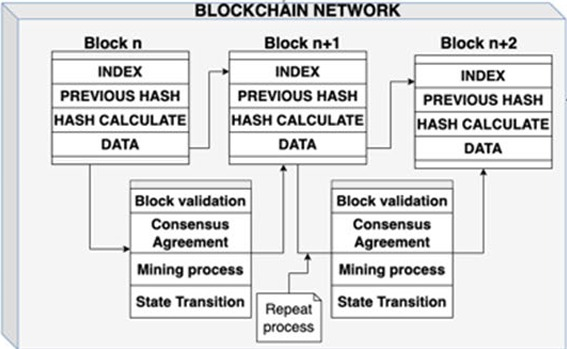
\includegraphics[width=0.85\textwidth]{figure/blockchain_network_architecture.png}
    \caption{Struktur rangkaian blok pada blockchain}
    \label{fig:blockchain_architecture}
    \vspace{2pt}
    {\footnotesize Sumber: diolah dari~\cite{Rustemi2023SLR}}
\end{figure}

\subsection{Permissioned Blockchain}
Berdasarkan hak partisipasinya, blockchain dibedakan menjadi \textit{permissionless blockchain} yang dapat diikuti siapa saja dan \textit{permissioned blockchain} yang pesertanya dibatasi serta dikenal identitasnya. Pada \textit{permissioned blockchain}, setiap peserta harus memiliki identitas yang diterbitkan pihak berwenang sebelum dapat membaca atau menulis data~\cite{FabricMSP}. Jenis ini banyak diusulkan untuk verifikasi dokumen akademik karena lembaga penerbit dapat mengatur siapa saja yang boleh menulis data~\cite{Pandari2026Blockchain,Blanco2025Digital}. Perkembangan penggunaan jenis platform blockchain pada penelitian verifikasi sertifikat akademik berdasarkan tahun publikasi ditunjukkan pada Gambar~\ref{fig:permissioned}.

\begin{figure}[H]
    \centering
    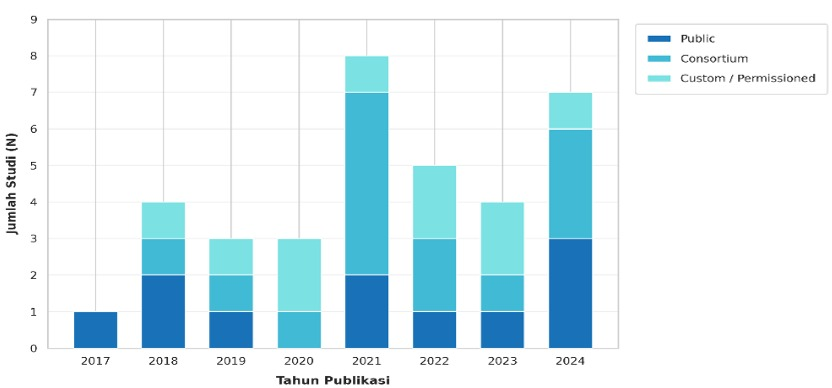
\includegraphics[width=0.85\textwidth]{figure/PermissionedBlockchain.png}
    \caption{Evolusi jenis platform blockchain berdasarkan tahun publikasi}
    \label{fig:permissioned}
    \vspace{2pt}
    {\footnotesize Sumber: diolah dari~\cite{Pandari2026Blockchain}}
\end{figure}

\subsection{Hyperledger Fabric}
Hyperledger Fabric adalah platform \textit{permissioned blockchain} sumber terbuka yang telah diterapkan untuk penerbitan dan verifikasi sertifikat akademik~\cite{Dash2025Hyperledger,Blanco2025Digital}. Identitas setiap peserta dikelola oleh \textit{Membership Service Provider} (MSP) dalam bentuk sertifikat X.509 dengan peran seperti \textit{client}, \textit{admin}, \textit{peer}, dan \textit{orderer}~\cite{FabricMSP}. Aplikasi klien mengirim usulan transaksi ke \textit{peer} untuk dieksekusi dan disahkan sesuai \textit{endorsement policy}~\cite{FabricEndorsement}, kemudian \textit{orderer} mengurutkan transaksi menjadi blok yang dikirim kembali ke setiap \textit{peer} untuk divalidasi dan dicatat ke \textit{ledger}. Karena \textit{ledger} disalin pada setiap \textit{peer}, catatan SKL tersimpan dalam lebih dari satu salinan. Arsitektur jaringan dan alur transaksi tersebut ditunjukkan pada Gambar~\ref{fig:fabric}.

\begin{figure}[H]
    \centering
    \begin{subfigure}[b]{0.85\textwidth}
        \centering
        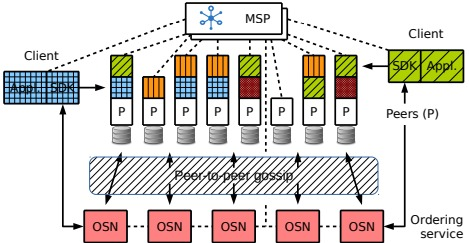
\includegraphics[width=\textwidth]{figure/ArsitekturjaringanHyperledgerFabric.png}
        \caption{Arsitektur jaringan}
        \label{fig:fabric_arsitektur}
    \end{subfigure}

    \vspace{6pt}
    \begin{subfigure}[b]{0.85\textwidth}
        \centering
        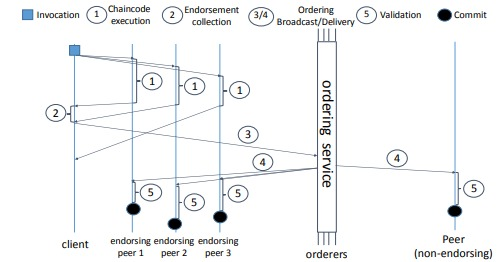
\includegraphics[width=\textwidth]{figure/AlurtransaksitingkattinggiHyperledgerFabric.png}
        \caption{Alur transaksi}
        \label{fig:fabric_alur}
    \end{subfigure}
    \vspace{2pt}
    \caption{Arsitektur dan alur transaksi Hyperledger Fabric}
    \label{fig:fabric}
    \vspace{2pt}
    {\footnotesize Sumber: diolah dari~\cite{FabricMSP,FabricEndorsement}}
\end{figure}

Komponen identitas dan otorisasi di Hyperledger Fabric saling berkaitan dalam satu rantai kepercayaan. \textit{Fabric Certificate Authority} (Fabric CA) mendaftarkan dan menerbitkan sertifikat X.509 bagi setiap pengguna dan \textit{node}; pada saat pendaftaran, atribut seperti \texttt{role=waka} dapat ditanamkan ke dalam sertifikat pengguna~\cite{FabricCA}. MSP kemudian menentukan CA mana yang dipercaya oleh suatu organisasi dan mengelompokkan setiap identitas ke dalam peran \textit{client}, \textit{peer}, \textit{admin}, atau \textit{orderer}, sehingga sertifikat yang tidak diterbitkan CA tersebut ditolak oleh jaringan~\cite{FabricMSP}. Setelah identitas dinyatakan sah oleh MSP, \textit{chaincode} membaca atribut peran pada sertifikat melalui pustaka cid untuk menegakkan kontrol akses berbasis atribut (ABAC)~\cite{FabricCID}. Terakhir, \textit{endorsement policy} menentukan \textit{peer} mana yang wajib mengeksekusi dan menandatangani hasil transaksi, dan transaksi yang pengesahannya tidak memenuhi kebijakan tersebut ditandai tidak valid saat validasi~\cite{FabricEndorsement}. Hubungan keempat komponen tersebut ditunjukkan pada Gambar~\ref{fig:relasi_fabric}.

\begin{figure}[H]
    \centering
    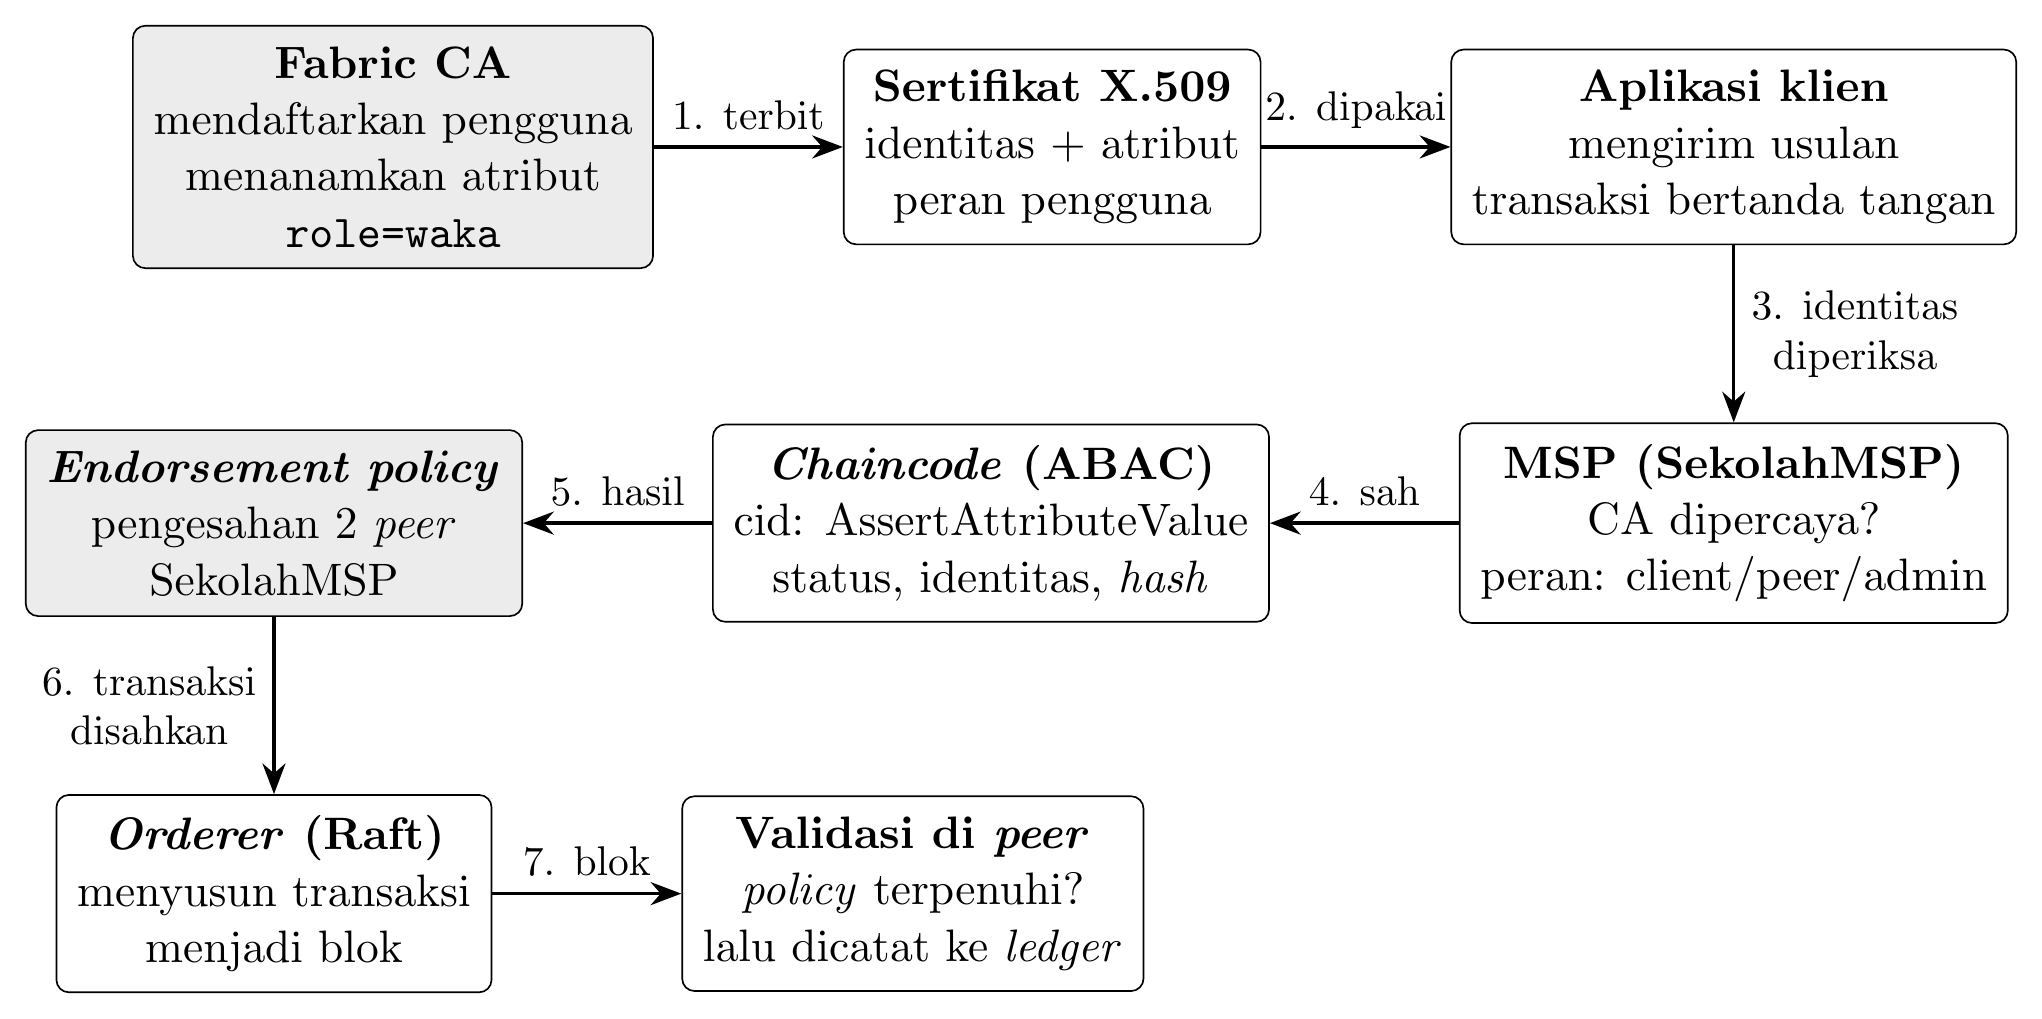
\includegraphics[width=0.85\textwidth]{figure/RelasiCA_MSP_ABAC_Endorsement.png}
    \caption{Hubungan Fabric CA, MSP, ABAC, dan \textit{endorsement policy}}
    \label{fig:relasi_fabric}
    \vspace{2pt}
    {\footnotesize Sumber: diolah dari~\cite{FabricCA,FabricMSP,FabricCID,FabricEndorsement}}
\end{figure}

Rancangan konfigurasi \textit{node}, \textit{channel}, dan \textit{endorsement policy} yang digunakan pada penelitian ini dijelaskan pada Subbab~\ref{III.Metode}.

\subsection{Smart Contract}
\textit{Smart contract} adalah program yang berjalan di jaringan blockchain dan menjalankan aturan secara otomatis ketika syarat tertentu terpenuhi. Pada Hyperledger Fabric, \textit{smart contract} disebut \textit{chaincode}, misalnya fungsi untuk membuat, memverifikasi, dan mencabut sertifikat seperti pada penelitian Dash dkk.~\cite{Dash2025Hyperledger}. Pada penelitian ini, \textit{chaincode} SKL mengatur setiap tahap penerbitan, pencabutan, dan kueri status, sehingga aturan kewenangan ditegakkan oleh jaringan, bukan hanya oleh aplikasi.

\subsection{Multi-Otoritas dan Kontrol Akses Berbasis Atribut}
Multi-otoritas adalah aturan bahwa suatu tindakan baru sah setelah disetujui lebih dari satu pihak berwenang, seperti pencabutan oleh minimal dua otoritas pada Tariq dkk.~\cite{Tariq2023Cerberus} dan pengesahan berjenjang pada Al Hemairy dkk.~\cite{AlHemairy2024UAE}. Aturan ini ditegakkan dengan kontrol akses berbasis atribut (\textit{attribute-based access control}, ABAC), yaitu hak akses ditentukan oleh atribut pengguna seperti perannya. Di Hyperledger Fabric, atribut peran ditanamkan pada sertifikat pengguna, lalu \textit{chaincode} membacanya melalui pustaka \textit{client identity} (cid) dengan fungsi seperti GetAttributeValue dan AssertAttributeValue~\cite{FabricCID}. Dengan demikian, setiap tahap hanya dapat dijalankan oleh peran yang berwenang dan sesuai urutannya, seperti ditunjukkan pada Gambar~\ref{fig:multiotoritas}.

\begin{figure}[H]
    \centering
    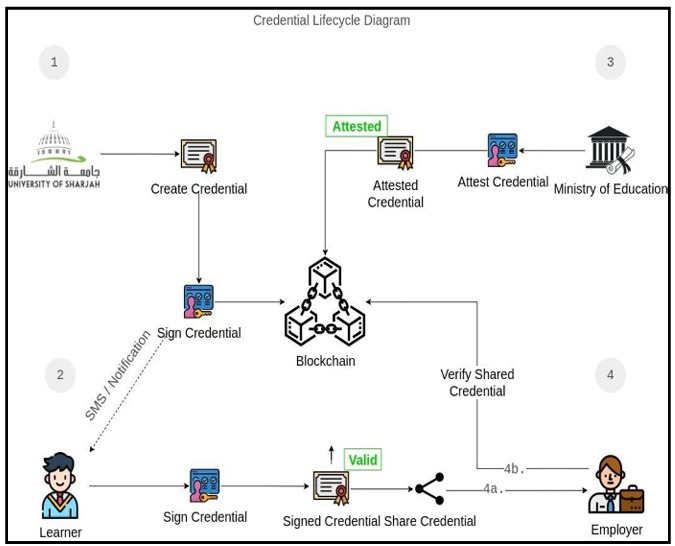
\includegraphics[width=0.85\textwidth]{figure/Multi-OtoritasdanKontrolAksesBerbasisAtribut.png}
    \caption{Siklus hidup kredensial dengan pengesahan berjenjang}
    \label{fig:multiotoritas}
    \vspace{2pt}
    {\footnotesize Sumber: Al Hemairy dkk.~\cite{AlHemairy2024UAE}}
\end{figure}

Secara umum terdapat tiga pola multi-otoritas. Pada persetujuan berurutan (\textit{sequential approval}), setiap otoritas menyetujui secara bergiliran dalam urutan tetap. Pada \textit{multi-signature}, beberapa tanda tangan dikumpulkan pada satu transaksi tanpa urutan, seperti pada Al Hemairy dkk.~\cite{AlHemairy2024UAE}. Pada persetujuan ambang (\textit{threshold approval}), tindakan sah apabila minimal $k$ dari $n$ otoritas menyetujui, seperti pencabutan oleh minimal dua otoritas pada Tariq dkk.~\cite{Tariq2023Cerberus}. Penelitian ini memakai persetujuan berurutan untuk penerbitan karena prosedur sekolah bertingkat dan setiap tingkat memeriksa hal yang berbeda, serta persetujuan ambang dua dari tiga pejabat untuk pencabutan agar pencabutan tidak sepihak tetapi tetap dapat dilakukan saat seorang pejabat berhalangan.

Pola multi-otoritas dapat diterapkan pada \textit{chaincode} sebagai mesin status (\textit{state machine}), yaitu model yang menyatakan setiap dokumen berada pada satu status tertentu dan hanya dapat berpindah ke status berikutnya melalui transisi yang diizinkan~\cite{Augenio2025StateTransition}. Setiap fungsi \textit{chaincode} hanya mengubah status apabila syarat transisinya terpenuhi, misalnya atribut peran pemanggil sesuai fungsi yang diperiksa dengan AssertAttributeValue, status dokumen saat ini sesuai urutan, dan identitas pemanggil yang dibaca dengan fungsi GetID belum pernah menyetujui dokumen tersebut~\cite{FabricCID}. Dengan cara ini, urutan persetujuan dan pemisahan tugas ditegakkan oleh jaringan, bukan hanya oleh aplikasi. Rancangan status, fungsi, dan transisi untuk SKL pada penelitian ini dijelaskan pada Subbab~\ref{III.Metode}.

Persetujuan berbasis peran tersebut berbeda dengan \textit{endorsement} oleh \textit{peer}. Persetujuan berbasis peran adalah keputusan pejabat sekolah yang dikirim sebagai transaksi terpisah untuk setiap tahap dan ditandatangani sertifikat pejabat yang bersangkutan, sehingga menjawab pertanyaan ``siapa yang berwenang menyetujui SKL''. \textit{Endorsement} adalah tanda tangan \textit{peer} atas hasil eksekusi \textit{chaincode} untuk setiap transaksi, termasuk setiap transaksi persetujuan, sehingga menjawab pertanyaan ``apakah hasil eksekusi transaksi ini sah dan konsisten''~\cite{FabricEndorsement}. Dengan demikian, dokumen yang memerlukan beberapa tahap persetujuan melewati satu transaksi untuk setiap tahap, dan setiap transaksi tersebut tetap disahkan oleh \textit{peer} sesuai \textit{endorsement policy}. Perbedaan keduanya dirangkum pada Tabel~\ref{table:2.endorsement}.

\begin{table}[H]
    \centering
    \caption{Perbedaan persetujuan berbasis peran dan \textit{endorsement peer}}
    \label{table:2.endorsement}
    \footnotesize
    \renewcommand{\arraystretch}{1.25}
    \begin{tabular}{|>{\raggedright\arraybackslash}p{0.18\textwidth}|>{\raggedright\arraybackslash}p{0.35\textwidth}|>{\raggedright\arraybackslash}p{0.35\textwidth}|}
        \hline
        \textbf{Aspek} & \textbf{Persetujuan berbasis peran} & \textbf{\textit{Endorsement peer}} \\
        \hline
        Pelaku & Pejabat sekolah melalui akun klien & \textit{Node peer} \\
        \hline
        Tujuan & Otorisasi: hanya peran berwenang, sesuai urutan & Konsistensi: hasil eksekusi \textit{chaincode} sama dan sah \\
        \hline
        Letak aturan & Logika \textit{chaincode} (atribut, status, identitas, \textit{hash}) & \textit{Endorsement policy} pada definisi \textit{chaincode} \\
        \hline
        Bukti & Transaksi per tahap yang ditandatangani sertifikat pejabat & Tanda tangan \textit{peer} atas hasil eksekusi \\
        \hline
        Jumlah & Satu transaksi untuk setiap tahap persetujuan & Sesuai jumlah \textit{peer} yang disyaratkan \textit{endorsement policy} untuk setiap transaksi \\
        \hline
        Jika gagal & Transaksi ditolak \textit{chaincode} dengan pesan kesalahan & Transaksi ditandai tidak valid saat validasi \\
        \hline
    \end{tabular}
\end{table}

\subsection{Surat Keterangan Lulus}
Surat Keterangan Lulus (SKL) adalah dokumen yang diterbitkan kepala satuan pendidikan pada tanggal penetapan kelulusan dan bersifat sementara sampai ijazah diterbitkan~\cite{Kepmendikdasmen2026SKL}. SKL memuat paling sedikit identitas peserta didik dan nilai rata-rata yang nantinya tercantum dalam transkrip nilai~\cite{Kepmendikdasmen2026SKL}. Karena memuat data anak, pemrosesan data SKL tunduk pada ketentuan pelindungan data pribadi yang menggolongkan data anak sebagai data pribadi spesifik~\cite{UU27Tahun2022}. Contoh format SKL ditunjukkan pada Gambar~\ref{fig:contoh_format_skl}.

\begin{figure}[H]
    \centering
    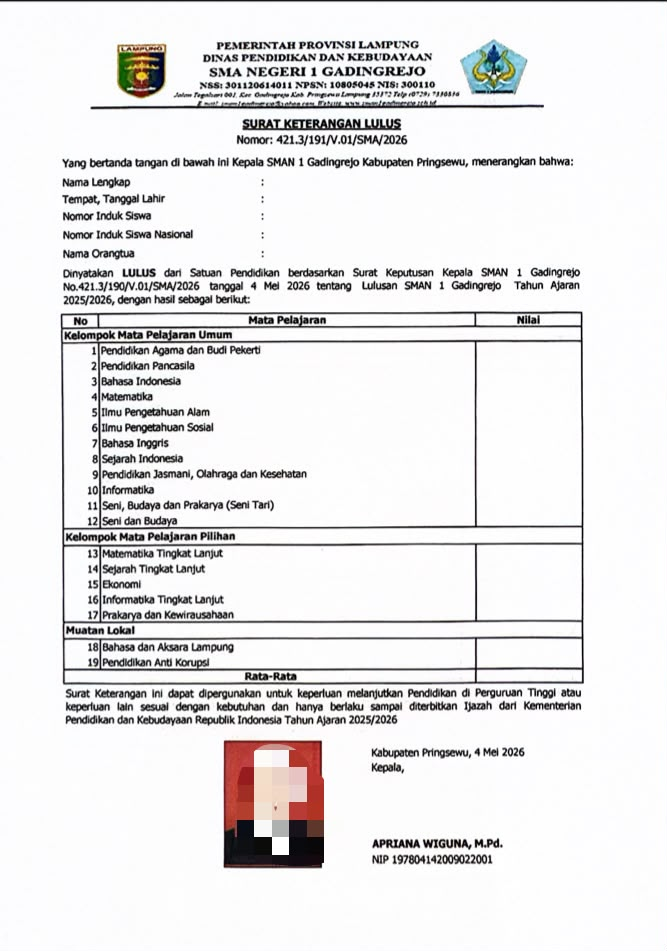
\includegraphics[width=0.85\textwidth]{figure/ContohFormatSKL.jpeg}
    \caption{Contoh Format SKL}
    \label{fig:contoh_format_skl}
    \vspace{2pt}
    {\footnotesize Sumber: SMAN 1 Gadingrejo (2026)}
\end{figure}

\subsection{Private Data Collection}
\textit{Private data collection} adalah fitur Hyperledger Fabric untuk menyimpan data rahasia hanya pada \textit{peer} yang berwenang, sedangkan \textit{peer} lain hanya menerima \textit{hash} data tersebut sebagai bukti transaksi~\cite{FabricPrivateData}. Data privat dapat dihapus (\textit{purge}) setelah sejumlah blok tertentu, sementara \textit{hash}-nya tetap tersimpan di \textit{ledger}~\cite{FabricPrivateData}. Pendekatan ini dipakai Blanco dkk.~\cite{Blanco2025Digital} agar data sensitif tetap berada di luar rantai. Pada penelitian ini, data lengkap SKL disimpan pada \textit{private data collection}, sedangkan \textit{ledger} hanya menyimpan ID SKL, nomor surat, \textit{hash}, status, identitas penulis transaksi, dan waktu transaksi, seperti ditunjukkan pada Gambar~\ref{fig:pdc_ledger}.

\begin{figure}[H]
    \centering
    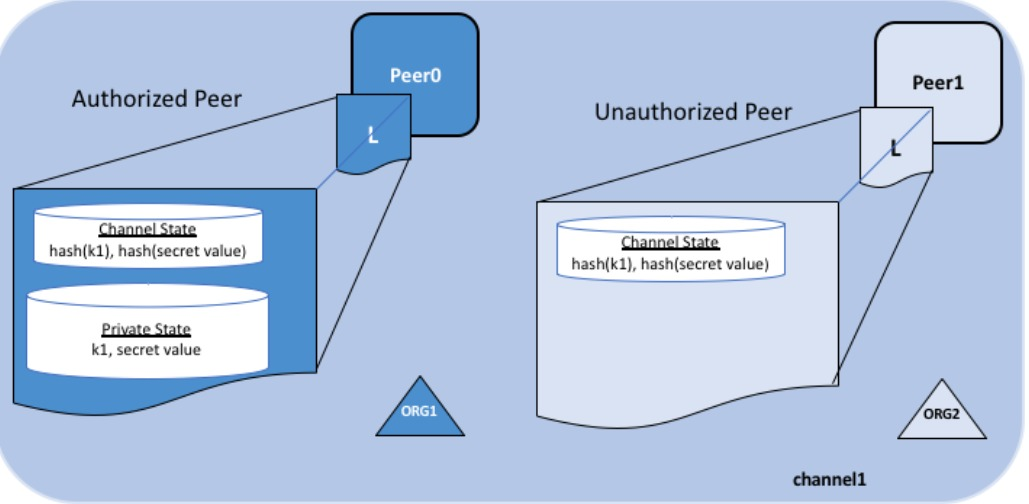
\includegraphics[width=0.85\textwidth]{figure/Isiledgerpadapeerberwenangdanpeertidakberwenangdalamprivatedatacollection.png}
    \caption{Isi ledger pada peer berwenang dan peer tidak berwenang dalam private data collection}
    \label{fig:pdc_ledger}
    \vspace{2pt}
    {\footnotesize Sumber: Hyperledger Foundation~\cite{FabricPrivateData}}
\end{figure}

Pengelolaan data pada \textit{private data collection} diatur melalui konfigurasi koleksi, antara lain \textit{policy} yang menentukan organisasi anggota koleksi, \textit{requiredPeerCount} dan \textit{maxPeerCount} yang menentukan jumlah \textit{peer} lain yang menerima data saat pengesahan, \textit{blockToLive} yang menentukan masa simpan data, serta \textit{memberOnlyRead} dan \textit{memberOnlyWrite} yang membatasi pembacaan dan penulisan hanya untuk anggota koleksi~\cite{FabricPrivateData}. Data privat dikirim aplikasi melalui \textit{transient field}, sehingga isi data tidak ikut tercatat pada usulan transaksi maupun blok, lalu disimpan oleh \textit{chaincode} ke basis data privat setiap \textit{peer} anggota koleksi~\cite{FabricPrivateData}. Rancangan konfigurasi koleksi untuk data SKL dijelaskan pada Subbab~\ref{III.Metode}.

\subsection{Fungsi Hash SHA-256}
Fungsi \textit{hash} mengubah data berukuran apa pun menjadi nilai berukuran tetap, dan perubahan sekecil apa pun pada data masukan menghasilkan nilai \textit{hash} yang berbeda~\cite{NIST2015FIPS1804}. SHA-256 menghasilkan nilai \textit{hash} 256 bit dan dipakai pada sistem verifikasi kredensial berbasis blockchain, misalnya pada Cerberus~\cite{Tariq2023Cerberus}. Prosesnya terdiri atas dua tahap, yaitu \textit{preprocessing} (penambahan \textit{padding}, pemecahan pesan menjadi blok 512 bit, dan penetapan nilai \textit{hash} awal) serta komputasi \textit{hash} yang memakai 64 \textit{word} jadwal pesan dan delapan variabel kerja 32 bit untuk setiap blok~\cite{NIST2015FIPS1804}, seperti ditunjukkan pada Gambar~\ref{fig:sha256_architecture}.

\begin{figure}[H]
    \centering
    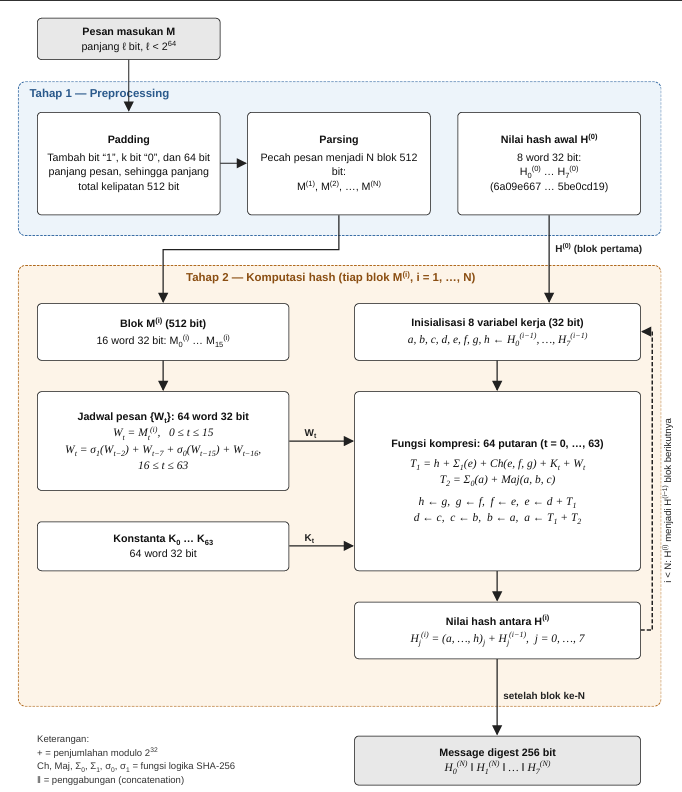
\includegraphics[width=0.85\textwidth]{figure/Arsitektur_fungsi_hash_SHA256.png}
    \caption{Arsitektur fungsi hash SHA-256}
    \label{fig:sha256_architecture}
    \vspace{2pt}
    {\footnotesize Sumber: diolah dari~\cite{NIST2015FIPS1804}}
\end{figure}

Pada penelitian ini, bukti integritas SKL yang dicatat di \textit{ledger} adalah nilai \textit{hash} dari data SKL yang dihitung dengan rumus berikut.
\begin{equationcaptioned}[eq:hash]{h_{SKL} = \mbox{SHA-256}\left(D_{SKL} \parallel s\right)}{Nilai \textit{hash} SKL}
\end{equationcaptioned}
\noindent
dengan $h_{SKL}$ adalah nilai \textit{hash} yang dicatat di \textit{ledger}, $D_{SKL}$ adalah data SKL yang disusun dalam bentuk baku (kanonik) dengan urutan \textit{field} tetap, $s$ adalah nilai acak (\textit{salt}) yang disimpan bersama data di \textit{private data collection}, dan $\parallel$ berarti penggabungan. Perubahan satu karakter saja pada $D_{SKL}$ menghasilkan $h_{SKL}$ yang berbeda, sehingga perubahan isi SKL dapat terdeteksi saat verifikasi~\cite{Dash2025Hyperledger,Blanco2025Digital}. \textit{Salt} ditambahkan karena data SKL relatif mudah ditebak (nama, NISN, dan nilai), sehingga tanpa \textit{salt} pihak yang hanya melihat \textit{hash} dapat mencoba menebak isinya.

Secara umum, keaslian dokumen diverifikasi dengan menghitung ulang nilai \textit{hash} dari data dokumen dan \textit{salt}, lalu membandingkannya dengan nilai \textit{hash} yang tercatat di \textit{ledger}~\cite{Blanco2025Digital}. Apabila kedua nilai sama, isi dokumen tidak berubah sejak dicatat; apabila berbeda, isi dokumen telah diubah. Karena yang dibandingkan hanya nilai \textit{hash}, verifikasi dapat dilakukan tanpa membuka data pribadi yang tersimpan di \textit{private data collection}. Rancangan pembangkitan \textit{salt} dan alur verifikasi SKL oleh pihak eksternal pada penelitian ini dijelaskan pada Subbab~\ref{III.Metode}.

\subsection{Black Box Testing}
\textit{Black box testing} atau \textit{behavioural testing} adalah metode pengujian perangkat lunak berdasarkan perilakunya, yaitu dengan memberikan masukan dan memeriksa keluaran tanpa melihat struktur kode program~\cite{Putri2024BlackBox}. Pada penelitian ini, \textit{black box testing} dipakai untuk menguji kontrol akses, yaitu memeriksa apakah setiap peran hanya dapat menjalankan fungsi \textit{chaincode} yang menjadi kewenangannya dan ditolak saat menjalankan fungsi di luar kewenangannya, seperti ditunjukkan pada Gambar~\ref{fig:blackbox_testing}.

\begin{figure}[H]
    \centering
    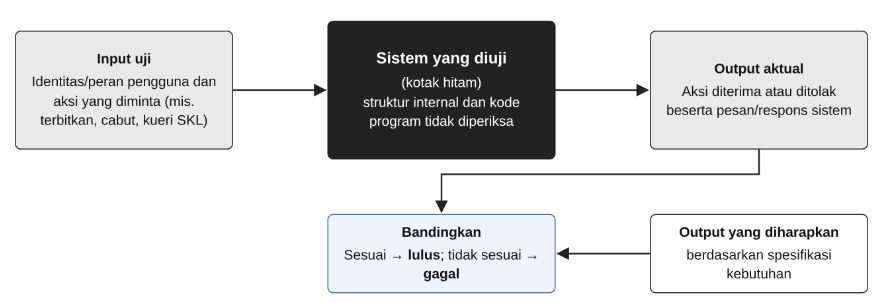
\includegraphics[width=0.85\textwidth]{figure/Konsepblackboxtestingpadapengujiankontrolakses.png}
    \caption{Konsep \textit{black box testing} pada pengujian kontrol akses}
    \label{fig:blackbox_testing}
    \vspace{2pt}
    {\footnotesize Sumber: diolah dari~\cite{Putri2024BlackBox}}
\end{figure}

Teknik \textit{black box testing} yang digunakan adalah \textit{state transition testing}, yaitu teknik yang menguji perpindahan sistem dari satu status ke status lain akibat suatu kejadian, termasuk memastikan perpindahan yang tidak sah ditolak~\cite{Augenio2025StateTransition}. Teknik ini sesuai karena aturan multi-otoritas diterapkan sebagai mesin status, dan Augenio dan Hardiyanti~\cite{Augenio2025StateTransition} melaporkan bahwa \textit{state transition testing} dapat mengeksekusi seluruh kasus uji dengan nilai \textit{Average Percentage of Fault Detection} lebih tinggi daripada \textit{equivalence class partitioning}. Setiap transisi yang sah diuji untuk memastikan diterima, sedangkan setiap transisi yang tidak sah diuji untuk memastikan ditolak. Rancangan skenario dan kasus uji \textit{state transition testing} pada penelitian ini dijelaskan pada Subbab~\ref{III.Pengujian}.

Hasil pengujian dinyatakan sebagai persentase skenario uji yang hasilnya sesuai dengan yang diharapkan, sebagaimana diterapkan pada pengujian \textit{black box} oleh Sakinah dkk.~\cite{Sakinah2024BlackBox}, dengan rumus berikut.
\begin{equationcaptioned}[eq:blackbox]{P = \frac{S_{sesuai}}{S_{total}} \times 100\%}{Persentase keberhasilan pengujian}
\end{equationcaptioned}
\noindent
dengan $P$ adalah persentase keberhasilan pengujian, $S_{sesuai}$ adalah jumlah skenario uji yang hasilnya sesuai harapan, dan $S_{total}$ adalah jumlah seluruh skenario uji. Misalnya, 34 skenario uji yang seluruhnya sesuai harapan menghasilkan persentase keberhasilan sebesar 100\%.

\subsection{Hyperledger Caliper}
Hyperledger Caliper adalah alat \textit{benchmark} untuk mengukur kinerja jaringan blockchain, termasuk Hyperledger Fabric~\cite{Caliper}. Caliper mengirim beban transaksi sesuai skenario, lalu melaporkan jumlah transaksi berhasil dan gagal, \textit{latency}, dan \textit{throughput}~\cite{Caliper}. Dash dkk.~\cite{Dash2025Hyperledger} memakai Caliper untuk membandingkan kinerja Hyperledger Fabric dengan Ethereum dan Bitcoin, sehingga hasil penelitian ini dapat dibandingkan dengan hasil tersebut. Alur pengujian dengan Caliper ditunjukkan pada Gambar~\ref{fig:caliper_architecture}.

\begin{figure}[H]
    \centering
    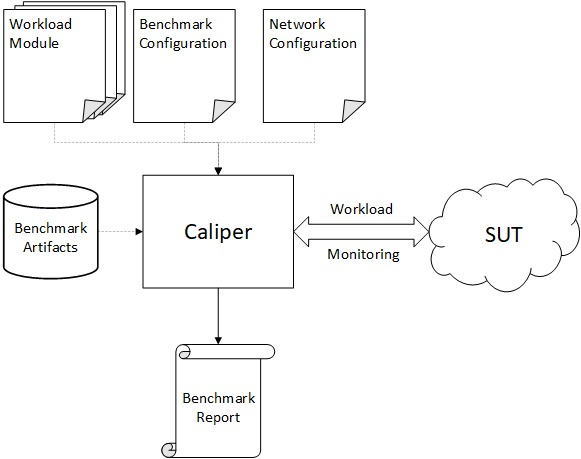
\includegraphics[width=0.85\textwidth]{figure/ArsitekturtingkattinggiHyperledgerCaliper.png}
    \caption{Arsitektur tingkat tinggi Hyperledger Caliper}
    \label{fig:caliper_architecture}
    \vspace{2pt}
    {\footnotesize Sumber:~\cite{Caliper}}
\end{figure}

\textit{Throughput} menyatakan jumlah transaksi yang berhasil dicatat jaringan per detik (TPS)~\cite{Caliper} dan dihitung dengan rumus berikut.
\begin{equationcaptioned}[eq:throughput]{\mathit{Throughput} = \frac{\sum \mbox{transaksi berhasil}}{\mbox{total waktu pengujian (detik)}}}{\textit{Throughput}}
\end{equationcaptioned}
\noindent
Transaksi yang gagal tidak dihitung dalam pembilang. Misalnya, 1.000 transaksi berhasil dalam 20 detik menghasilkan \textit{throughput} sebesar 50 TPS.

\textit{Latency} menyatakan waktu yang dibutuhkan sejak transaksi dikirim sampai transaksi selesai dicatat jaringan~\cite{Caliper} dan dihitung dengan rumus berikut.
\begin{equationcaptioned}[eq:latency]{\mathit{Latency} = t_{selesai} - t_{kirim}}{\textit{Latency}}
\end{equationcaptioned}
\noindent
dengan $t_{kirim}$ adalah waktu transaksi dikirim dan $t_{selesai}$ adalah waktu transaksi tercatat. Caliper melaporkan nilai rata-rata, minimum, dan maksimum dari seluruh transaksi.

\textit{Success rate} menyatakan persentase transaksi yang berhasil dari seluruh transaksi yang dikirim~\cite{Caliper} dan dihitung dengan rumus berikut.
\begin{equationcaptioned}[eq:successrate]{\mathit{Success\ rate} = \frac{Succ}{Succ + Fail} \times 100\%}{\textit{Success rate}}
\end{equationcaptioned}
\noindent
dengan $Succ$ adalah jumlah transaksi berhasil dan $Fail$ adalah jumlah transaksi gagal yang dilaporkan Caliper. Misalnya, 990 transaksi berhasil dan 10 transaksi gagal menghasilkan \textit{success rate} sebesar 99\%.

\textit{Overhead} multi-otoritas adalah tambahan waktu yang dibutuhkan untuk menerbitkan satu dokumen melalui beberapa tahap persetujuan dibandingkan penerbitan oleh satu otoritas. Waktu penerbitan satu dokumen dihitung sebagai jumlah \textit{latency} seluruh transaksi yang diperlukan dokumen tersebut, yang diukur dengan Caliper~\cite{Caliper}, dan pola satu otoritas digunakan sebagai pembanding seperti pada Dash dkk.~\cite{Dash2025Hyperledger}. \textit{Overhead} multi-otoritas dihitung dengan rumus berikut.
\begin{equationcaptioned}[eq:overhead]{O = \frac{\bar{L}_{B} - \bar{L}_{A}}{\bar{L}_{A}} \times 100\%}{\textit{Overhead} multi-otoritas}
\end{equationcaptioned}
\noindent
dengan $O$ adalah \textit{overhead} multi-otoritas, $\bar{L}_{A}$ adalah rata-rata waktu penerbitan satu dokumen oleh satu otoritas (skenario A), dan $\bar{L}_{B}$ adalah rata-rata waktu penerbitan satu dokumen melalui multi-otoritas (skenario B). Misalnya, apabila $\bar{L}_{A}$ sebesar 0,5 detik dan $\bar{L}_{B}$ sebesar 2,1 detik, maka \textit{overhead} multi-otoritas sebesar 320\%. Angka ini menunjukkan tambahan waktu sebagai biaya keamanan dari persetujuan bertingkat.

\subsection{Metode Prototyping}
Metode \textit{prototyping} adalah metode pengembangan perangkat lunak yang membangun versi awal sistem secara cepat, memperlihatkannya kepada pengguna, lalu memperbaikinya berdasarkan umpan balik sampai sesuai kebutuhan~\cite{Adim2025Prototype}. Metode ini terdiri atas lima tahap, yaitu \textit{communication} untuk mengumpulkan kebutuhan, \textit{quick plan} untuk menyusun rencana singkat, \textit{modeling quick design} untuk membuat rancangan cepat, \textit{construction of prototype} untuk membangun prototipe, serta \textit{deployment, delivery}, dan \textit{feedback} untuk menyerahkan prototipe dan menerima umpan balik pengguna~\cite{Adim2025Prototype}. Apabila prototipe belum sesuai, tahapan diulang mulai dari \textit{communication}. Metode ini sesuai untuk penelitian ini karena aturan kewenangan penerbitan SKL perlu dikonfirmasi langsung kepada pihak sekolah dan dapat berubah setelah sekolah melihat prototipe.

\begin{figure}[H]
    \centering
    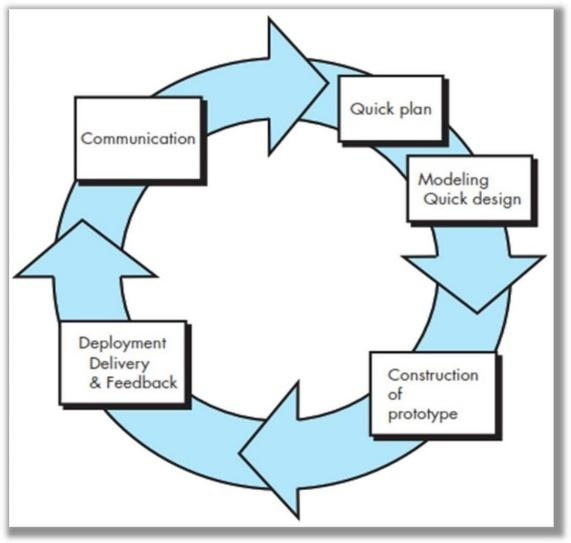
\includegraphics[width=0.55\textwidth]{figure/ModelPrototyping.png}
    \caption{Model \textit{prototyping}}
    \label{fig:model_prototyping}
    \vspace{2pt}
    {\footnotesize Sumber: Adim dkk.~\cite{Adim2025Prototype}}
\end{figure}